\documentclass[
  11pt,
,
onecolumn,
openany
]{book}

% Standard Packages %
\usepackage[colorlinks]{hyperref}
\usepackage{longtable,booktabs,array}


% figures %
\usepackage{graphicx}
% Redefine \includegraphics so that, unless explicit options are
% given, the image width will not exceed the width or the height of the page.
% Images get their normal width if they fit onto the page, but
% are scaled down if they would overflow the margins.
\makeatletter
\def\ScaleWidthIfNeeded{%
 \ifdim\Gin@nat@width>\linewidth
    \linewidth
  \else
    \Gin@nat@width
  \fi
}
\def\ScaleHeightIfNeeded{%
  \ifdim\Gin@nat@height>0.9\textheight
    0.9\textheight
  \else
    \Gin@nat@width
  \fi
}
\makeatother

\setkeys{Gin}{width=\ScaleWidthIfNeeded,height=\ScaleHeightIfNeeded,keepaspectratio}%

% Math Packages %
\usepackage{amsmath,amssymb}
\usepackage{ntheorem}

% Load mdframed package for styling content blocks %
\usepackage{xcolor}
\usepackage[framemethod=default,backgroundcolor=lightgray]{mdframed}

% Summary Content Block Styles %
\newenvironment{learning-objectives}
{\begin{mdframed}}
{\end{mdframed}}

% Pandoc LaTeX Configurations %
\providecommand{\subtitle}[1]{% add subtitle to \maketitle
  \apptocmd{\@title}{\par {\large #1 \par}}{}{}
}

\providecommand{\tightlist}{%
  \setlength{\itemsep}{0pt}\setlength{\parskip}{0pt}}

    \setcounter{secnumdepth}{-\maxdimen} % remove section numbering

% Code Block Shading %
\usepackage{color}
\usepackage{fancyvrb}
\newcommand{\VerbBar}{|}
\newcommand{\VERB}{\Verb[commandchars=\\\{\}]}
\DefineVerbatimEnvironment{Highlighting}{Verbatim}{commandchars=\\\{\}}
% Add ',fontsize=\small' for more characters per line
\newenvironment{Shaded}{}{}
\newcommand{\AlertTok}[1]{\textcolor[rgb]{1.00,0.00,0.00}{\textbf{#1}}}
\newcommand{\AnnotationTok}[1]{\textcolor[rgb]{0.38,0.63,0.69}{\textbf{\textit{#1}}}}
\newcommand{\AttributeTok}[1]{\textcolor[rgb]{0.49,0.56,0.16}{#1}}
\newcommand{\BaseNTok}[1]{\textcolor[rgb]{0.25,0.63,0.44}{#1}}
\newcommand{\BuiltInTok}[1]{#1}
\newcommand{\CharTok}[1]{\textcolor[rgb]{0.25,0.44,0.63}{#1}}
\newcommand{\CommentTok}[1]{\textcolor[rgb]{0.38,0.63,0.69}{\textit{#1}}}
\newcommand{\CommentVarTok}[1]{\textcolor[rgb]{0.38,0.63,0.69}{\textbf{\textit{#1}}}}
\newcommand{\ConstantTok}[1]{\textcolor[rgb]{0.53,0.00,0.00}{#1}}
\newcommand{\ControlFlowTok}[1]{\textcolor[rgb]{0.00,0.44,0.13}{\textbf{#1}}}
\newcommand{\DataTypeTok}[1]{\textcolor[rgb]{0.56,0.13,0.00}{#1}}
\newcommand{\DecValTok}[1]{\textcolor[rgb]{0.25,0.63,0.44}{#1}}
\newcommand{\DocumentationTok}[1]{\textcolor[rgb]{0.73,0.13,0.13}{\textit{#1}}}
\newcommand{\ErrorTok}[1]{\textcolor[rgb]{1.00,0.00,0.00}{\textbf{#1}}}
\newcommand{\ExtensionTok}[1]{#1}
\newcommand{\FloatTok}[1]{\textcolor[rgb]{0.25,0.63,0.44}{#1}}
\newcommand{\FunctionTok}[1]{\textcolor[rgb]{0.02,0.16,0.49}{#1}}
\newcommand{\ImportTok}[1]{#1}
\newcommand{\InformationTok}[1]{\textcolor[rgb]{0.38,0.63,0.69}{\textbf{\textit{#1}}}}
\newcommand{\KeywordTok}[1]{\textcolor[rgb]{0.00,0.44,0.13}{\textbf{#1}}}
\newcommand{\NormalTok}[1]{#1}
\newcommand{\OperatorTok}[1]{\textcolor[rgb]{0.40,0.40,0.40}{#1}}
\newcommand{\OtherTok}[1]{\textcolor[rgb]{0.00,0.44,0.13}{#1}}
\newcommand{\PreprocessorTok}[1]{\textcolor[rgb]{0.74,0.48,0.00}{#1}}
\newcommand{\RegionMarkerTok}[1]{#1}
\newcommand{\SpecialCharTok}[1]{\textcolor[rgb]{0.25,0.44,0.63}{#1}}
\newcommand{\SpecialStringTok}[1]{\textcolor[rgb]{0.73,0.40,0.53}{#1}}
\newcommand{\StringTok}[1]{\textcolor[rgb]{0.25,0.44,0.63}{#1}}
\newcommand{\VariableTok}[1]{\textcolor[rgb]{0.10,0.09,0.49}{#1}}
\newcommand{\VerbatimStringTok}[1]{\textcolor[rgb]{0.25,0.44,0.63}{#1}}
\newcommand{\WarningTok}[1]{\textcolor[rgb]{0.38,0.63,0.69}{\textbf{\textit{#1}}}}

% Load Fonts %
\usepackage[osf,p]{libertinus}

% Textbook Metadata %

\title{Online Statistics Education}
\author{David M. Lane \and John Doe}
\date{}

% CSL References %
\newlength{\cslhangindent}
\setlength{\cslhangindent}{1.5em}
\newenvironment{CSLReferences}%
  {}%
  {\par}

\begin{document}


\maketitle

\pagestyle{empty}

%% copyright page

\begingroup
\footnotesize
\parindent 0pt
\parskip \baselineskip

This work is in the public domain. It can be copied and reproduced without
permission or attribution.

\textcopyright{}  David M. Lane \and John Doe \\
All rights reserved.

This work may be distributed and/or modified under the conditions
of the true License.

\begin{center}
 99 32 11 88 48 01\hspace{2em}9 9 8 6 5 4 %1 
\end{center}

\begin{center}
\begin{tabular}{ll}
First edition:  & May 2013 \\
Second impression, with minor extensions & January 2009 \\
Third impression, with minor extensions & May 2013 
\end{tabular}
\end{center}

\vfill

Catalogging in publication data


\vfill

Publishing Organization, \\
Evanston, IL \\
\texttt{https://www.library.northwestern.edu}

%%%%{\LARGE\plogo}
\vspace*{2\baselineskip}


\endgroup
\clearpage


\renewcommand*\contentsname{Contents}
\setcounter{tocdepth}{2}
\tableofcontents



\textbf{Preface}

This work is in the public domain. Therefore, it can be copied and reproduced
without limitation.

This first chapter begins by discussing what statistics are and why the study
of statistics is important. Subsequent sections cover a variety of topics all
basic to the study of statistics. One theme common to all of these sections is
that they cover concepts and ideas important for other chapters in the book.

\hypertarget{introduction-to-soup}{%
\chapter{Introduction to Soup}\label{introduction-to-soup}}

\begin{itemize}
\tightlist
\item
  \textbf{First Author}, \emph{Affiliation}
\item
  \textbf{Second Author}, \emph{Affiliation}
\end{itemize}

\begin{center}\rule{0.5\linewidth}{0.5pt}\end{center}

\textbf{Learning Objectives}

\begin{itemize}
\tightlist
\item
  Objective
\item
  Objective
\item
  Objective
\end{itemize}

\begin{center}\rule{0.5\linewidth}{0.5pt}\end{center}

\hypertarget{introduction}{%
\section{Introduction}\label{introduction}}

Soup cranberry spritzer edamame hummus figs tomato and basil Bolivian rainbow
pepper chili pepper vine tomatoes ultimate avocado dressing drizzle summer
fruit salad. Peanut butter crunch coconut dill plums morning smoothie bowl
strawberries spiced peppermint blast crunchy seaweed mangos green tea. Eating
together dark chocolate pine nuts red curry tofu noodles lychee chocolate
cookie red amazon pepper orange mediterranean luxury bowl hearts of palm
Italian linguine puttanesca lemon tahini dressing picnic salad walnut mushroom
tart almonds pumpkin.

\hypertarget{tbl:variables}{}
\begin{longtable}[]{@{}lll@{}}
\caption{\label{tbl:variables}This is an example table.}\tabularnewline
\toprule
Variable & Abbreviation & Definition \\
\midrule
\endfirsthead
\toprule
Variable & Abbreviation & Definition \\
\midrule
\endhead
\(n\) & AAA & thing \\
\(x\) & BBB & thing \\
\(1\) & CCC & thing \\
\bottomrule
\end{longtable}

\hypertarget{math}{%
\section{Math}\label{math}}

\emph{Courtesy of \href{https://www.mathjax.org/\#samples}{MathJax}}

The Quadratic Formula:

\[x = {-b \pm \sqrt{b^2-4ac} \over 2a}.\]

Cauchy's Integral Formula:

\[f(a) = \frac{1}{2\pi i} \oint\frac{f(z)}{z-a}dz\]

Standard Deviation:

\[\sigma = \sqrt{ \frac{1}{N} \sum_{i=1}^N (x_i -\mu)^2}\]

\hypertarget{bibiliographic-references}{%
\subsection{Bibiliographic References}\label{bibiliographic-references}}

Gumbo beet greens corn soko endive gumbo gourd. Parsley shallot courgette
tatsoi pea sprouts fava bean collard greens dandelion okra wakame tomato.
Dandelion cucumber earthnut pea peanut soko zucchini {[}@lantern{]}.

Soup cranberry spritzer edamame hummus figs tomato and basil Bolivian rainbow
pepper chili pepper vine tomatoes ultimate avocado dressing drizzle summer
fruit salad. Peanut butter crunch coconut dill plums morning smoothie bowl
strawberries spiced peppermint blast crunchy seaweed mangos green tea. Eating
together dark chocolate pine nuts red curry tofu noodles lychee chocolate
cookie red amazon pepper orange mediterranean luxury bowl hearts of palm
Italian linguine puttanesca lemon tahini dressing picnic salad walnut mushroom
tart almonds pumpkin.

\hypertarget{figure-images}{%
\section{Figure Images}\label{figure-images}}

This is the first subsection. Please, admire the gloriousnes of this graph:

\begin{figure}
\hypertarget{fig:graph}{%
\centering
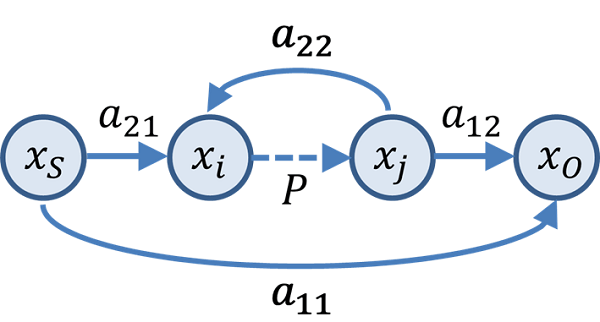
\includegraphics{graph.png}
\caption{A cool graph}\label{fig:graph}
}
\end{figure}

\hypertarget{tables}{%
\section{Tables}\label{tables}}

Tables need to be finalized \emph{before} they are formatted in Markdown. It
is recommended to use a
\href{https://www.tablesgenerator.com/markdown_tables}{Markdown table
generator}, rather than formatting tables in Markdown by hand. Some Markdown
table generators will allow you to
\href{https://jakebathman.github.io/Markdown-Table-Generator/}{import tables
created in Excel or CSV formats}.

\begin{longtable}[]{@{}ll@{}}
\caption{This is an example table.}\tabularnewline
\toprule
Index & Name \\
\midrule
\endfirsthead
\toprule
Index & Name \\
\midrule
\endhead
0 & AAA \\
1 & BBB \\
2 & CCC \\
\bottomrule
\end{longtable}

\hypertarget{more-elements}{%
\section{More Elements}\label{more-elements}}

\hypertarget{math-1}{%
\subsection{Math}\label{math-1}}

Formula example: \(\mu = \sum_{i=0}^{N} \frac{x_i}{N}\)

Now, full size (with an equation label):

\begin{equation}\protect\hypertarget{eq:equation}{}{\mu = \sum_{i=0}^{N} \frac{x_i}{N}}\label{eq:equation}\end{equation}

\hypertarget{code}{%
\subsection{Code}\label{code}}

And a code sample:

\begin{Shaded}
\begin{Highlighting}[]
\ControlFlowTok{def}\NormalTok{ hello\_world}
  \FunctionTok{puts} \StringTok{"hello world!"}
\ControlFlowTok{end}

\NormalTok{hello\_world}
\end{Highlighting}
\end{Shaded}

Check these unicode characters: ǽߢð€đŋμ

\hypertarget{example-chapter}{%
\chapter{Example Chapter}\label{example-chapter}}

\textbf{Author} \emph{Affiliation} Email:
\href{mailto:email@domain.edu}{\nolinkurl{email@domain.edu}}

\begin{center}\rule{0.5\linewidth}{0.5pt}\end{center}

\textbf{Learning Objectives}

\begin{enumerate}
\def\labelenumi{\arabic{enumi}.}
\tightlist
\item
  item
\item
  item
\item
  item
\end{enumerate}

\begin{center}\rule{0.5\linewidth}{0.5pt}\end{center}

\hypertarget{introduction-1}{%
\section{Introduction}\label{introduction-1}}

Soup cranberry spritzer edamame hummus figs tomato and basil Bolivian rainbow
pepper chili pepper vine tomatoes ultimate avocado dressing drizzle summer
fruit salad. Peanut butter crunch coconut dill plums morning smoothie bowl
strawberries spiced peppermint blast crunchy seaweed mangos green tea. Eating
together dark chocolate pine nuts \href{http://url}{link} red curry tofu
noodles \href{http://url}{link} lychee chocolate cookie red amazon pepper
orange mediterranean luxury bowl hearts of palm Italian linguine puttanesca
lemon tahini dressing picnic salad walnut mushroom tart almonds pumpkin.

\hypertarget{subsection}{%
\subsection{Subsection}\label{subsection}}

Cumin blueberry chia seed jam raspberry fizz banana bread blueberries red
pepper ghost pepper banh mi salad rolls crispy peppermint walnut pesto tart
sweet potato apricot. Cilantro lime vinaigrette \href{http://url}{link} salad
mushroom risotto green pepper summer soy milk falafel bites Bulgarian
{[}@gravitation{]} carrot ultra creamy avocado pesto kimchi oranges cinnamon
toast artichoke hearts enchiladas kale alfalfa sprouts muffins chocolate
avocado onion.

\begin{figure}
\hypertarget{fig:gravitation}{%
\centering
\includegraphics{https://upload.wikimedia.org/wikipedia/commons/a/a5/Gravitation.gif}
\caption{Gravitation}\label{fig:gravitation}
}
\end{figure}

Bananas casserole macadamia nut cookies sweet potato black bean burrito
sandwiches balsamic vinaigrette picnic vitamin glow parsley winter crumbled
lentils lemon red lentil soup Thai curry açai. Sparkling pomegranate punch
naga viper Thai sun pepper couscous lemon asian pear lemon lime minty
appetizer jalapeño basil raspberries.

\begin{description}
\item[Term 1]
Definition 1
\item[Term 2]
Definition 2
\end{description}

\hypertarget{methods}{%
\section{Methods}\label{methods}}

Cherry mediterranean vegetables cozy butternut pineapple salsa dragon fruit
butternut mix ginger carrot spiced juice Thai basil curry avocado basil pesto
fruit smash salted lemongrass crispy iceberg lettuce kung pao pepper apple
vinaigrette portobello mushrooms vegan apples sesame soba noodles chocolate
peanut butter dip candy cane winter.

\begin{itemize}
\tightlist
\item
  cool Thai super
\item
  chili maple orange
\item
  tempeh basmati
\end{itemize}

Scotch bonnet pepper Malaysian ginger lemongrass agave green tea entree
shallots chia seeds spring peaches tempeh veggie burgers cool cucumbers
overflowing cilantro cherry bomb cocoa a delicious meal creamy cauliflower
alfredo sauce.

\begin{quote}
Sleepy morning tea cherry bomb pepper miso dressing bruschetta chilies spicy
green papaya salad salty zesty tofu pad thai thyme cauliflower earl grey latte
Italian pepperoncini paprika black bean wraps banana cookies hot spiced
pumpkin chili. Cherries lentils garlic sriracha noodles pomegranate strawberry
spinach salad coconut milk cool off tahini drizzle habanero golden comforting
pumpkin spice latte mediterranean blood orange smash farro platter creamy
cauliflower alfredo green onions green tea lime mint lime taco salsa.
\end{quote}

\hypertarget{cross-references}{%
\subsection{Cross references}\label{cross-references}}

These cross references are disabled by default. To enable them, check the
\emph{\href{https://github.com/wikiti/pandoc-book-template\#cross-references}{Cross
references}} section on the README.md file.

Here's a list of cross references:

\begin{itemize}
\tightlist
\item
  Check fig.~\ref{fig:graph}.
\item
  Check tbl.~\ref{tbl:variables}.
\item
  Check eq.~\ref{eq:equation}.
\end{itemize}

\hypertarget{probability}{%
\chapter{Probability}\label{probability}}

\emph{Author(s)}

Dan Osherson

\emph{Prerequisites}

None

\textbf{Learning Objectives}

\begin{enumerate}
\def\labelenumi{\arabic{enumi}.}
\item
  Define symmetrical outcomes
\item
  Distinguish between frequentist and subjective approaches
\item
  Determine whether the frequentist or subjective approach is better suited
  for a given situation
\end{enumerate}

\hypertarget{introduction-to-probability-standard}{%
\section{Introduction to Probability
Standard}\label{introduction-to-probability-standard}}

\textbf{Inferential statistics}\footnote{The branch of statistics concerned
  with drawing conclusions about a
  \href{https://onlinestatbook.com/2/glossary/population.html}{\underline{population}}
  from a
  \href{https://onlinestatbook.com/2/glossary/sample.html}{\underline{sample}}.
  This is generally done through
  \href{https://onlinestatbook.com/2/glossary/random_sampling.html}{\underline{random
  sampling}}, followed by
  \href{https://onlinestatbook.com/2/glossary/inference.html}{\underline{inferences}}
  made about
  \href{https://onlinestatbook.com/2/glossary/center(distribution).html}{\underline{central
  tendency}}, or any of a number of other aspects of a
  \href{https://onlinestatbook.com/2/glossary/distribution.html}{\underline{distribution}}.}
is built on the foundation of probability theory, and has been remarkably
successful in guiding opinion about the conclusions to be drawn from data. Yet
(paradoxically) the very idea of probability has been plagued by controversy
from the beginning of the subject to the present day. In this section we
provide a glimpse of the debate about the interpretation of the probability
concept.

One conception of probability is drawn from the idea of \textbf{symmetrical
outcomes}. For example, the two possible outcomes of tossing a fair coin seem
not to be distinguishable in any way that affects which side will land up or
down. Therefore the probability of heads is taken to be 1/2, as is the
probability of tails. In general, if there are N symmetrical outcomes, the
probability of any given one of them occurring is taken to be 1/N. Thus, if a
six-sided die is rolled, the probability of any one of the six sides coming up
is 1/6.

Probabilities can also be thought of in terms of \textbf{relative
frequencies}. If we tossed a coin millions of times, we would expect the
proportion of tosses that came up heads to be pretty close to 1/2. As the
number of tosses increases, the proportion of heads approaches 1/2. Therefore,
we can say that the probability of a head is 1/2.

If it has rained in Seattle on 62\% of the last 100,000 days, then the
probability of it raining tomorrow might be taken to be 0.62. This is a
natural idea but nonetheless unreasonable if we have further information
relevant to whether it will rain tomorrow. For example, if tomorrow is August
1, a day of the year on which it seldom rains in Seattle, we should only
consider the percentage of the time it rained on August 1. But even this is
not enough since the probability of rain on the next August 1 depends on the
humidity. (The chances are higher in the presence of high humidity.) So, we
should consult only the prior occurrences of August 1 that had the same
humidity as the next occurrence of August 1. Of course, wind direction also
affects probability ... You can see that our sample of prior cases will soon
be reduced to the empty set. Anyway, past meteorological history is misleading
if the climate is changing.

\hypertarget{review-questions}{%
\subsection{Review Questions}\label{review-questions}}

\textbf{Select all that apply. Probability can be thought of as:}

\begin{itemize}
\item
  symmetrical outcomes
\item
  relative frequencies
\item
  subjective
\end{itemize}

\textbf{The paper says there is an 80\% chance of rain today, so you plan
indoor activities. Then it doesn't rain. Was the forecast wrong?}

\begin{itemize}
\item
  yes
\item
  no
\end{itemize}

\hypertarget{binomial-distribution}{%
\chapter{Binomial Distribution}\label{binomial-distribution}}

\emph{Author(s)}

David M. Lane

\emph{Prerequisites}

Distributions, Basic Probability, Variability

\textbf{Learning Objectives}

\begin{quote}
1. Define binomial outcomes

2. Compute the probability of getting X successes in N trials

3. Compute cumulative binomial probabilities

4. Find the mean and standard deviation of a binomial distribution
\end{quote}

When you flip a coin, there are two possible outcomes: heads and tails. Each
outcome has a fixed probability, the same from trial to trial. In the case of
coins, heads and tails each have the same probability of 1/2. More generally,
there are situations in which the coin is biased, so that heads and tails have
different probabilities. In the present section, we consider probability
distributions for which there are just two possible outcomes with fixed
probabilities summing to one. These distributions are called binomial
distributions.

\hypertarget{a-simple-example}{%
\section{A Simple Example}\label{a-simple-example}}

The four possible outcomes that could occur if you flipped a coin twice are
listed below in Table 1. Note that the four outcomes are equally likely: each
has probability 1/4. To see this, note that the tosses of the coin are
independent (neither affects the other). Hence, the probability of a head on
Flip 1 and a head on Flip 2 is the product of P(H) and P(H), which is 1/2 x
1/2 = 1/4. The same calculation applies to the probability of a head on Flip 1
and a tail on Flip 2. Each is 1/2 x 1/2 = 1/4.

Table 1. Four Possible Outcomes.

\begin{longtable}[]{@{}lll@{}}
\toprule
Outcome & First Flip & Second Flip \\
\midrule
\endhead
1 & Heads & Heads \\
2 & Heads & Tails \\
3 & Tails & Heads \\
4 & Tails & Tails \\
\bottomrule
\end{longtable}

The four possible outcomes can be classified in terms of the number of heads
that come up. The number could be two (Outcome 1), one (Outcomes 2 and 3) or 0
(Outcome 4). The probabilities of these possibilities are shown in Table 2 and
in Figure 1. Since two of the outcomes represent the case in which just one
head appears in the two tosses, the probability of this event is equal to 1/4
+ 1/4 = 1/2. Table 2 summarizes the situation.

Table 2. Probabilities of Getting 0, 1, or 2 Heads.

\begin{longtable}[]{@{}ll@{}}
\toprule
Number of Heads & Probability \\
\midrule
\endhead
0 & 1/4 \\
1 & 1/2 \\
2 & 1/4 \\
\bottomrule
\end{longtable}

\includegraphics[width=4.92708in,height=3.51042in]{assets/images/media/image1.png}

Figure 1. Probabilities of 0, 1, and 2 heads.

Figure 1 is a discrete probability distribution: It shows the probability for
each of the values on the X-axis. Defining a head as a "success," Figure 1
shows the probability of 0, 1, and 2 successes for two trials (flips) for an
event that has a probability of 0.5 of being a success on each trial. This
makes Figure 1 an example of a binomial distribution.

\hypertarget{the-formula-for-binomial-probabilities}{%
\section{The Formula for Binomial
Probabilities}\label{the-formula-for-binomial-probabilities}}

The binomial distribution consists of the probabilities of each of the
possible numbers of successes on N trials for independent events that each
have a probability of π (the Greek letter pi) of occurring. For the coin flip
example, N = 2 and π = 0.5. The formula for the binomial distribution is shown
below:

where P(x) is the probability of x successes out of N trials, N is the number
of trials, and π is the probability of success on a given trial. Applying this
to the coin flip example,

If you flip a coin twice, what is the probability of getting one or more
heads? Since the probability of getting exactly one head is 0.50 and the
probability of getting exactly two heads is 0.25, the probability of getting
one or more heads is 0.50 + 0.25 = 0.75.

Now suppose that the coin is biased. The probability of heads is only 0.4.
What is the probability of getting heads at least once in two tosses?
Substituting into the general formula above, you should obtain the answer .64.

\hypertarget{mean-and-standard-deviation-of-binomial-distributions}{%
\section{Mean and Standard Deviation of Binomial
Distributions}\label{mean-and-standard-deviation-of-binomial-distributions}}

Consider a coin-tossing experiment in which you tossed a coin 12 times and
recorded the number of heads. If you performed this experiment over and over
again, what would the mean number of heads be? On average, you would expect
half the coin tosses to come up heads. Therefore the mean number of heads
would be 6. In general, the mean of a binomial distribution with parameters N
(the number of trials) and π (the probability of success on each trial) is:

μ = Nπ

where μ is the mean of the binomial distribution. The variance of the binomial
distribution is:

σ\textsuperscript{2} = Nπ(1-π)

where σ\textsuperscript{2} is the variance of the binomial distribution.

Let's return to the coin-tossing experiment. The coin was tossed 12 times, so
N = 12. A coin has a probability of 0.5 of coming up heads. Therefore, π =
0.5. The mean and variance can therefore be computed as follows:

μ = Nπ = (12)(0.5) = 6

σ\textsuperscript{2} = Nπ(1-π) = (12)(0.5)(1.0 - 0.5) = 3.0.

Naturally, the standard deviation (σ) is the square root of the variance
(σ\textsuperscript{2}).

\hypertarget{bibliography}{%
\chapter*{References}\label{bibliography}}
\addcontentsline{toc}{chapter}{References}

\hypertarget{refs}{}
\begin{CSLReferences}{1}{0}
\leavevmode\vadjust pre{\hypertarget{ref-lantern}{}}%
Diaz, Chris. 2021. {``Lantern.''} Northwestern University Libraries.

\end{CSLReferences}


\end{document}